%%%%%%%%%%%%%%%%%%%%%%%%%%%%%%%%%%%%

\section{Inference for other estimators}

%%%%%%%%%%%%%%%%%%%%%%%%%%%%%%%%%%%%

\begin{frame}
\frametitle{Inference for other estimators}

\begin{itemize}

\item The sample mean is not the only point estimate for which the sampling distribution is nearly normal. For example, the sampling distribution of sample proportions is also nearly normal when $n$ is sufficiently large.

\item An important assumption about point estimates is that they are \hl{unbiased}, i.e. the sampling distribution of the estimate is centered at the true population parameter it estimates. 
\begin{itemize}
\item That is, an unbiased estimate does not naturally over or underestimate the parameter. Rather, it tends to provide a ``good" estimate. 
\item The sample mean is an example of an unbiased point estimate, as are each of the examples we introduce in this section.
\end{itemize}

\item Some point estimates follow distributions other than the normal distribution, and some scenarios require statistical techniques that we haven't covered yet -- we will discuss these at the end of this section.

\end{itemize}

\end{frame}

%%%%%%%%%%%%%%%%%%%%%%%%%%%%%%%%%%%%

\subsection{Confidence intervals for nearly normal point estimates}

%%%%%%%%%%%%%%%%%%%%%%%%%%%%%%%%%%%%

\begin{frame}
\frametitle{Confidence intervals for nearly normal point estimates}

A confidence interval based on an unbiased and nearly normal point estimate is

\[ point~estimate � z^\star SE \]

where $z^\star$ is selected to correspond to the confidence level, and SE represents the standard error. 

$\:$ \\

Remember that the value $z^\star SE$ is called the \hl{margin of error}.

\end{frame}

%%%%%%%%%%%%%%%%%%%%%%%%%%%%%%%%%%%

\begin{frame}
\frametitle{}

{\small
\pq{One of the earliest examples of behavioral asymmetry is a preference in humans for turning the head to the right, rather than to the left, during the final weeks of gestation and for the first 6 months after birth. This is thought to influence subsequent development of perceptual and motor preferences. A study of 124 couples found that 64.5\% turned their heads to the right when kissing. The standard error associated with this estimate is roughly 4\%. Which of the below is \emph{false}?}
\begin{enumerate}[(a)]
\solnMult{The 95\% confidence interval for the percentage of kissers who turn their heads to the right is roughly $64.5\% \pm 4\%$.}
\item A higher sample size would yield a lower standard error.
\item The margin of error for a 95\% confidence interval for the percentage of kissers who turn their heads to the right is roughly 8\%.
\item The 99.7\% confidence interval for the percentage of kissers who turn their heads to the right is roughly $64.5\% \pm 12\%$.
\end{enumerate}
}

\vfill

\ct{G\"{u}nt\"{u}rk\"{u}n, O. (2003) Adult persistence of head-turning asymmetry. \textit{Nature}. Vol 421.}

\end{frame}

%%%%%%%%%%%%%%%%%%%%%%%%%%%%%%%%%%%%

\subsection{Hypothesis testing for nearly normal point estimates}

%%%%%%%%%%%%%%%%%%%%%%%%%%%%%%%%%%%

\begin{frame}
\frametitle{Hypothesis testing for nearly normal point estimates}

\dq{The third National Health and Nutrition Examination Survey collected body fat percentage (BF\%) and gender data from 13,601 subjects ages 20 to 80. The average BF\% for the 6,580 men in the sample was 23.9, and this value was 35.0 for the 7,021 women. The standard error for the difference between the average men and women BF\%s was 0.114. Do these data provide convincing evidence that men and women have different average BF\%s. You may assume that the distribution of the point estimate is nearly normal.}

\pause

\begin{enumerate}
\item[1.] Set hypotheses
\item[2.] Calculate point estimate
\item[3.] Check conditions
\item[4.] Draw sampling distribution, shade p-value
\item[5.] Calculate test statistics and p-value, make a decision
\end{enumerate}

\end{frame}

%%%%%%%%%%%%%%%%%%%%%%%%%%%%%%%%%%%

\begin{frame}
\frametitle{}

\begin{enumerate}

\item[1.] The null hypothesis is that men and women have equal average BF\%, and the alternative is that these values are different.
\[ H_0: \mu_{men} = \mu_{women} \qquad H_A: \mu_{men} \ne \mu_{women} \]

\pause

\item [2.]The parameter of interest is the average difference in the population means of BF\%s for men and women, and the point estimate for this parameter is the difference between the two sample means:
\[ \bar{x}_{men} - \bar{x}_{women} = 23.9 - 35.0 = -11.1 \]

\pause

\item[3.] We are assuming that the distribution of the point estimate is nearly normal (we will discuss details for checking this condition in the next chapter, however given the large sample sizes, the normality assumption doesn't seem unwarranted).

\end{enumerate}


\end{frame}

%%%%%%%%%%%%%%%%%%%%%%%%%%%%%%%%%%%

\begin{frame}
\frametitle{}

\begin{enumerate}

\item[4.] The sampling distribution will be centered at the null value ($\mu_{men} - \mu_{women} = 0$), and the p-value is the area beyond the observed difference in sample means in both tails (lower than -11.1 and higher than 11.1).

\begin{center}
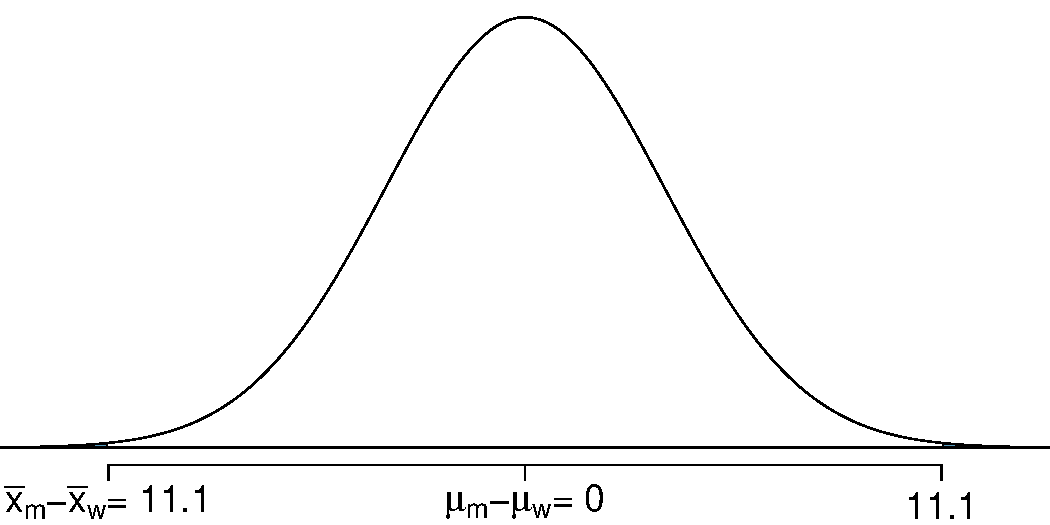
\includegraphics[width=0.75\textwidth]{4-5_inf_other_est/figures/bf/bf}
\end{center}


\end{enumerate}

\end{frame}

%%%%%%%%%%%%%%%%%%%%%%%%%%%%%%%%%%%

\begin{frame}
\frametitle{}

\begin{enumerate}

\item[5.] The test statistic is computed as the difference between the point estimate and the null value (-11.1 - 0 = -11.1), scaled by the standard error.

\[ Z = \frac{11.1 - 0}{0.114} = 97.36 \]

The Z score is huge! And hence the p-value will be tiny, allowing us to reject $H_0$ in favor of $H_A$.

\pause

$\:$ \\

These data provide convincing evidence that the average BF\% of men and women are different.

\end{enumerate}

\end{frame}

%%%%%%%%%%%%%%%%%%%%%%%%%%%%%%%%%%%

\subsection{Non-normal point estimates}

%%%%%%%%%%%%%%%%%%%%%%%%%%%%%%%%%%%

\begin{frame}
\frametitle{Non-normal point estimates}

\begin{itemize}

\item We may apply the ideas of confidence intervals and hypothesis testing to cases where the point estimate or test statistic is not necessarily normal. There are many reasons why such a situation may arise:
\begin{itemize}
\item the sample size is too small for the normal approximation to be valid;
\item the standard error estimate may be poor; or
\item the point estimate tends towards some distribution that is not the normal distribution.
\end{itemize}

\item For each case where the normal approximation is not valid, our first task is always to understand and characterize the sampling distribution of the point estimate or test statistic. Next, we can apply the general frameworks for confidence intervals and hypothesis testing to these alternative distributions.

\end{itemize}

\end{frame}

%%%%%%%%%%%%%%%%%%%%%%%%%%%%%%%%%%%

\subsection{When to retreat}

%%%%%%%%%%%%%%%%%%%%%%%%%%%%%%%%%%%

\begin{frame}
\frametitle{When to retreat}

\begin{itemize}

\item Statistical tools rely on the following two main conditions:
\begin{itemize}
\item \hlGr{Independence} A random sample from less than 10\% of the population ensures independence of observations. In experiments, this is ensured by random assignment. If independence fails, then advanced techniques must be used, and in some such cases, inference may not be possible.
\item \hlGr{Sample size and skew} For example, if the sample size is too small, the skew too strong, or extreme outliers are present, then the normal model for the sample mean will fail.
\end{itemize}

\item Whenever conditions are not satisfied for a statistical technique:
\begin{enumerate}
\item Learn new methods that are appropriate for the data. 
\item Consult a statistician.
\item \sout{Ignore the failure of conditions.} This last option effectively invalidates any analysis and may discredit novel and interesting findings.
\end{enumerate}

\end{itemize}

\end{frame}

%%%%%%%%%%%%%%%%%%%%%%%%%%%%%%%%%%%

\subsection{Statistical significance versus practical significance}

%%%%%%%%%%%%%%%%%%%%%%%%%%%%%%%%%%%

\begin{frame}
\frametitle{}

\pq{All else held equal, will the p-value be lower if $n = 100$ or $n = 10,000$?}

\begin{enumerate}[(a)]
\item $n = 100$
\solnMult{$n = 10,000$}
\end{enumerate}

\soln{\pause \pause
Suppose $\bar{x} = 50$, $s = 2$, $H_0: \mu = 49.5$, and $H_A: \mu > 49.5$.\\
\pause
\begin{eqnarray*}
Z_{n = 100} &=& \frac{50 - 49.5}{\frac{2}{\sqrt{100}}} \pause = \frac{50 - 49.5}{\frac{2}{10}} = \frac{0.5}{0.2} = 2.5,~~~\text{p-value} = 0.0062 \\
\pause
Z_{n = 10000} &=& \frac{50 - 49.5}{\frac{2}{\sqrt{10000}}} \pause = \frac{50 - 49.5}{\frac{2}{100}} = \frac{0.5}{0.02} = 25,~~~\text{p-value} \approx 0
\end{eqnarray*}
\pause
\begin{center}
As $n$ increases - $SE$ $\downarrow$, $Z$ $\uparrow$, p-value $\downarrow$
\end{center}
}

\end{frame}

%%%%%%%%%%%%%%%%%%%%%%%%%%%%%%%%%%%%

\begin{frame}

\dq{Test the hypothesis $H_0: \mu = 10$ vs. $H_A: \mu > 10$ for the following 8 samples. Assume $\sigma = 2$.}

\begin{center}
\renewcommand\arraystretch{1.5}
\begin{tabular}{l | c | c | c | c}
\hline
$\bar{x}$		& $10.05$ 	& $10.1$ 		& $10.2$  		 \\ 
\hline
\hline
\orange{$n = 30$}  
	& \soln{\only<1>{\textcolor{white}{$p-value = 0.45$}}		\only<2->{$p-value = 0.45$}}	
	& \soln{\only<1-3>{\textcolor{white}{$p-value = 0.39$}}		\only<4->{$p-value = 0.39$}} 		
	& \soln{\only<1-5>{\textcolor{white}{$p-value = 0.29$}}		\only<6->{$p-value = 0.29$}} \\
\hline
\hline
\orange{$n = 5000$} 
	& \soln{\only<1-2>{\textcolor{white}{$p-value = 0.39$}}		\only<3->{$p-value = 0.04$}}	
	& \soln{\only<1-4>{\textcolor{white}{$p-value = 0.0002$}}		\only<5->{$p-value = 0.0002$}}	
	& \soln{\only<1-6>{\textcolor{white}{$p-value \approx 0$}}	\only<7->{$p-value \approx 0$}}	 \\
\hline
\end{tabular}
\end{center}

\pause

\soln{\only<8->{When $n$ is large, even small deviations from the null (small effect sizes), which may be considered practically insignificant, can yield statistically significant results.}}

\end{frame}

%%%%%%%%%%%%%%%%%%%%%%%%%%%%%%%%%%%%

\begin{frame}
\frametitle{Statistical vs. practical significance}

\begin{itemize}

\item Real differences between the point estimate and null value are easier to detect with larger samples.

\item However, very large samples will result in statistical significance even for tiny differences between the sample mean and the null value (\hl{effect size}), even when the difference is not practically significant.

\item This is especially important to research: if we conduct a study, we want to focus on finding meaningful results (we want observed differences to be real, but also large enough to matter).

\item The role of a statistician is not just in the analysis of data, but also in planning and design of a study.
\end{itemize}

\begin{center}{\footnotesize
\textit{``To call in the statistician after the experiment is done may be no more than asking him to perform a post-mortem examination: he may be able to say what the experiment died of.''} -- R.A. Fisher
}\end{center}

\end{frame}

%%%%%%%%%%%%%%%%%%%%%%%%%%%%%%%%%%%%